\documentclass[14pt,a4paper]{extarticle}

% Page style
\usepackage[top=2cm,bottom=2cm,left=2cm,left=2cm,right=2cm,bindingoffset=0cm]{geometry}
% 1.3 means 1.5 =)
\linespread{1.3}
\usepackage{indentfirst}
\usepackage{hyperref}

% Useful packages
% Listings
\usepackage{minted}
% Figures
\usepackage{graphicx}
\usepackage{svg}
% Math
\usepackage{amsmath}
% Algorithm
\usepackage{algorithm,algorithmicx,algpseudocode}
% For long environments support page breaks
\usepackage{caption}

% Russian language and font
\usepackage[T2A]{fontenc}
\usepackage[english,russian]{babel}
\usepackage[mono=false]{libertine}
\usepackage{hyphenat}
\hyphenation{ма-те-ма-ти-ка вос-ста-нав-ли-вать}
\usepackage{csquotes}
\addto\captionsrussian{
	\renewcommand{\figurename}{Рисунок}
	\renewcommand{\partname}{Глава}
	\renewcommand{\contentsname}{Содержание}
	\renewcommand\listingscaption{Листинг}
}

% Bibliographies
\usepackage{biblatex}
\addbibresource{main.bib}

% Useful commands
\newcommand{\asection}[1]{
	\section*{#1}
	\addcontentsline{toc}{section}{#1}
}
% Break page free listing environment 
\newenvironment{code}{\captionsetup{type=listing}}{}

\begin{document}
\begin{titlepage}
	\begin{center}
		Министерство науки и высшего образования РФ\\
		Федеральное государственное бюджетное учреждение высшего образования\\
		Тверской государственный технический университет\\
		(ТвГТУ)\\
		Факультет информационных технологий\\
		Кафедра Программное обеспечение
		\vspace{6cm}

		Название предмета\\
		Отчёт по лабораторной работе №1\\
		Тема работы
		\vspace{3cm}

		\begin{flushright}
			\begin{minipage}{0.25\textwidth}
				\begin{flushleft}

					Работу выполнил:\\
					Малов А. В. \\
					Группа: Б.ПИН-РИС-20.06\\

					Проверил:\\
					% старший преподаватель кафедры ПО
					Иванов И. И.

				\end{flushleft}
			\end{minipage}
		\end{flushright}

		\vfill
		Тверь

		\the\year{}
	\end{center}
\end{titlepage}
\newpage

\tableofcontents
\newpage

\asection{Введение}

I know one book \cite{west2004}.

Привет, мир!

Lorem ipsum dolor sit amet, officia excepteur ex fugiat reprehenderit enim
labore culpa sint ad nisi Lorem pariatur mollit ex esse exercitation amet. Nisi
anim cupidatat excepteur officia. Reprehenderit nostrud nostrud ipsum Lorem est
aliquip amet voluptate voluptate dolor minim nulla est proident. Nostrud
officia pariatur ut officia. Sit irure elit esse ea nulla sunt ex occaecat
reprehenderit commodo officia dolor Lorem duis laboris cupidatat officia
voluptate. Culpa proident adipisicing id nulla nisi laboris ex in Lorem sunt
duis officia eiusmod. Aliqua reprehenderit commodo ex non excepteur duis sunt
velit enim. Voluptate laboris sint cupidatat ullamco ut ea consectetur et est
culpa et culpa duis.

\begin{code}
	\inputminted[fontsize=\footnotesize]{python}{listings/matrix.py}
	\caption{Some listing}
\end{code}

\begin{figure}[H]
	\begin{center}
		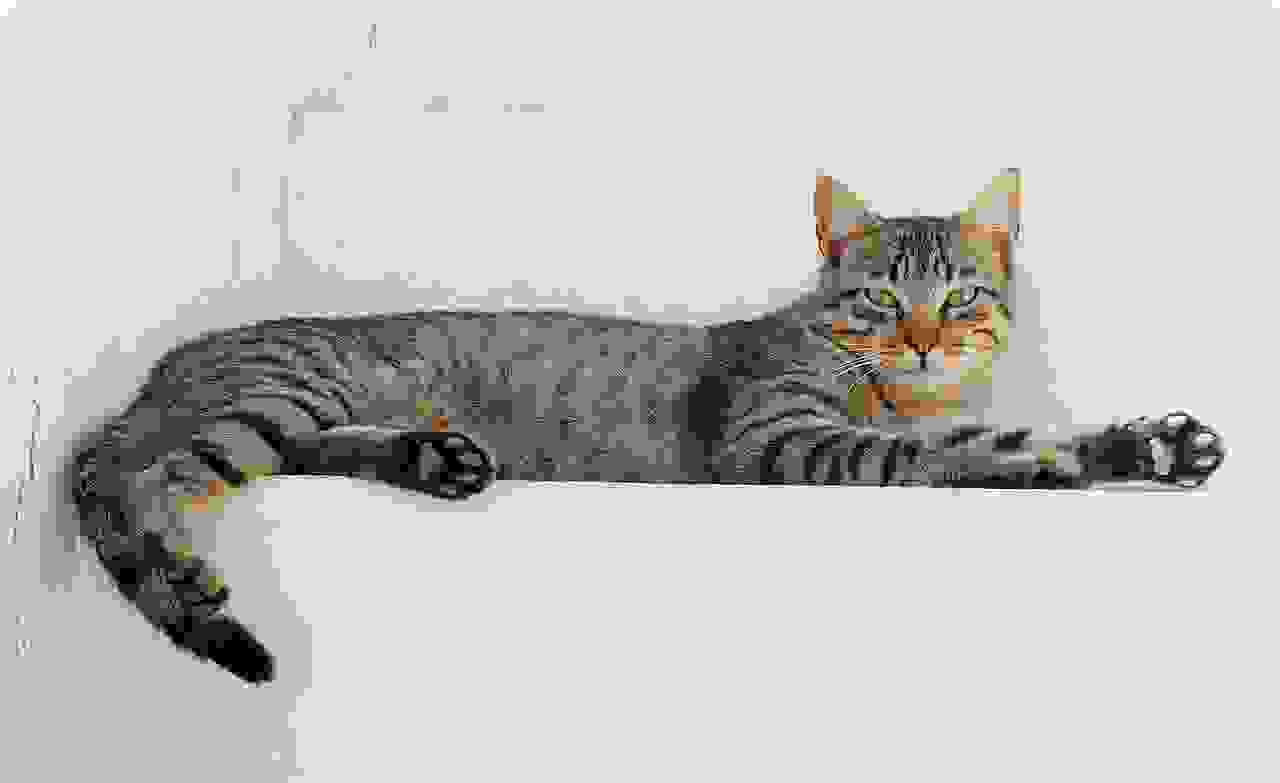
\includegraphics[width=0.95\textwidth]{figures/cat.jpg}
	\end{center}
	\caption{Some figure}
\end{figure}

\section{Глава с нумерацией}

Lorem ipsum dolor sit amet, qui minim labore adipisicing minim sint cillum sint
consectetur cupidatat.

\asection{Заключение}

Lorem ipsum dolor sit amet, officia excepteur ex fugiat reprehenderit enim
labore culpa sint ad nisi Lorem pariatur mollit ex esse exercitation amet. Nisi
anim cupidatat excepteur officia. Reprehenderit nostrud nostrud ipsum Lorem est
aliquip amet voluptate voluptate dolor minim nulla est proident. Nostrud
officia pariatur ut officia. Sit irure elit esse ea nulla sunt ex occaecat
reprehenderit commodo officia dolor Lorem duis laboris cupidatat officia
voluptate. Culpa proident adipisicing id nulla nisi laboris ex in Lorem sunt
duis officia eiusmod. Aliqua reprehenderit commodo ex non excepteur duis sunt
velit enim. Voluptate laboris sint cupidatat ullamco ut ea consectetur et est
culpa et culpa duis.

\newpage
\printbibliography[title={Список используемой литературы}]
\addcontentsline{toc}{section}{Список используемой литературы}

\end{document}

